%%%%%%%%%%%%%%%%%%%%
%%% Document
%%%%%%%%%%%%%%%%%%%%
\documentclass[pdftex, a4paper,11pt, twoside, ngerman]{report}
% \documentclass[11pt,xcolor=dvipsnames]{beamer}

% für deutsche zeichen äüö ohne kile auto-ersetzen
% \usepackage[utf8x]{inputenc}

% kile auto-ersetzen: einstellungen->latex:general-> hacken bei special
% characters
% \usepackage[ansinew]{inputenc}
% \usepackage[UKenglish]{babel}          %Englisch
\usepackage[ngerman]{babel}          %Deutsch


%%%%%%%%%%
%%% Geometry
%%%%%%%%%%
% \usepackage{showframe}
\usepackage[scale=0.8, hmarginratio=4:2]{geometry}
  \geometry{textheight=1.05\textheight, textwidth=.95\textwidth,
            marginparwidth=25 pt}



%%%%%%%%%%
%%% Packages (aus header datei)
%%%%%%%%%%
\IfFileExists{header_TobiasBrauell-DOCUMENT.tex}{
    % Copyright © 2014 Tobias Brauell <tobiasbrauell@gmail.com>

% This is my general purpose LaTeX header file for writing German documents.
% Ideally, you include this using a simple ``\input{header.tex}`` in your main
% document and start with ``\title`` and ``\begin{document}`` afterwards.

% If you need to add additional packages, I recommend not doing this in this
% file, but in your main document. That way, you can just drop in a new
% ``header.tex`` and get all the new commands without having to merge manually.

%%%%%%%%%%%%%%%%%%%%%%%%%%%%%
%%% Locale, date
%%%%%%%%%%%%%%%%%%%%%%%%%%%%%
\usepackage[UKenglish]{isodate}



%%%%%%%%%%%%%%%%%%%%%%%%%%%%%
%%% Margins and other spacing
%%%%%%%%%%%%%%%%%%%%%%%%%%%%%
\usepackage[activate]{pdfcprot}
% \usepackage[parfill]{parskip}
\usepackage{setspace}
  \setlength{\columnsep}{2 cm}
  \setlength{\parindent}{0 pt}


%%%%%%%%%%%%%%%%%%%%%%%%%%%%%
%%% Input encoding
%%%%%%%%%%%%%%%%%%%%%%%%%%%%%
\usepackage[T1]{fontenc}
\usepackage[utf8x]{inputenc}



%%%%%%%%%%%%%%%%%%%%%%%%%%%%%
%%% Indexing
%%%%%%%%%%%%%%%%%%%%%%%%%%%%%
\usepackage{makeidx}
  \makeindex



%%%%%%%%%%%%%%%%%%%%%%%%%%%%%
%%% Blindtext
%%%%%%%%%%%%%%%%%%%%%%%%%%%%%
\usepackage{blindtext}


%%%%%%%%%%%%%%%%%%%%%%%%%%%%%
%%% Global Counter
%%%%%%%%%%%%%%%%%%%%%%%%%%%%%



%%%%%%%%%%%%%%%%%%%%%%%%%%%%%
%%% Geometry
%%%%%%%%%%%%%%%%%%%%%%%%%%%%%
\usepackage{layout}
% \usepackage[scale=0.8]{geometry}
%   \geometry{textheight=1.05\textheight, marginparwidth=50 pt}

% \usepackage{multirow}
% \usepackage{dcolumn}



%%%%%%%%%%%%%%%%%%%%%%%%%%%%%
%%% Pagestyle
%%%%%%%%%%%%%%%%%%%%%%%%%%%%%
% \usepackage{fancyhdr}
% \usepackage{microtype} 

% \pagestyle{fancy}



%%%%%%%%%%%%%%%%%%%%%%%%%%%%%
%%% Fonts/Colors
%%%%%%%%%%%%%%%%%%%%%%%%%%%%%
\usepackage{lmodern}
\usepackage{xcolor}
% This replaces all fonts with Bitstream Charter, Bitstream Vera Sans and
% Bitstream Vera Mono. Math will be rendered in Charter.
% \usepackage[charter, greekuppercase=italicized]{mathdesign}
% \usepackage{beramono}
% \usepackage{berasans}

% Bold, sans-serif tensors. This fragment is taken from “egreg” from
% http://tex.stackexchange.com/a/82747/8945 and licensed under `CC-BY-SA
% <https://creativecommons.org/licenses/by-sa/3.0/>`_.
% \usepackage{bm}
%   \DeclareMathAlphabet{\mathsfit}{\encodingdefault}{\sfdefault}{m}{sl}
%   \SetMathAlphabet{\mathsfit}{bold}{\encodingdefault}{\sfdefault}{bx}{sl}
%   \newcommand{\tens}[1]{\bm{\mathsfit{#1}}}

% Bold vectors.
% \renewcommand{\vec}[1]{\boldsymbol{#1}}



%%%%%%%%%%%%%%%%%%%%%%%%%%%%%
%%% Code/Listings
%%%%%%%%%%%%%%%%%%%%%%%%%%%%%
\usepackage{listings}



%%%%%%%%%%%%%%%%%%%%%%%%%%%%%
%%% Enumerations
%%%%%%%%%%%%%%%%%%%%%%%%%%%%%
\usepackage{enumitem}
% \usepackage{paralist}


%%%%%%%%%%%%%%%%%%%%%%%%%%%%%
%%% Figures
%%%%%%%%%%%%%%%%%%%%%%%%%%%%%
% \usepackage[pdftex]{graphicx}
\usepackage{graphicx}
\usepackage{epsfig}
\usepackage{epstopdf}
\usepackage{subfigure}
\usepackage{wrapfig}
\makeatletter \newcommand\hyper@makecurrent[1]{} \makeatother
\usepackage{caption}
% \usepackage{subcaption}

\addto\captionsUKenglish{\renewcommand{\figurename}{Fig.}}
\addto\captionsngerman{\renewcommand{\figurename}{Abb.}}



%%%%%%%%%%%%%%%%%%%%%%%%%%%%%
%%% PDF Pages
%%%%%%%%%%%%%%%%%%%%%%%%%%%%%
\usepackage{pdfpages}



%%%%%%%%%%%%%%%%%%%%%%%%%%%%%
%%% Personal Graphics
%%%%%%%%%%%%%%%%%%%%%%%%%%%%%
\usepackage{tikz}
% \usepackage{tikz-3dplot}
  \usetikzlibrary{calc}
  \usetikzlibrary{decorations.markings}



%%%%%%%%%%%%%%%%%%%%%%%%%%%%%
%%% Math
%%%%%%%%%%%%%%%%%%%%%%%%%%%%%
\usepackage{amsmath}
\usepackage{amssymb}
\usepackage{mathtools}
\usepackage{dcolumn}
\usepackage{siunitx}
% \usepackage{feynmf}



%%%%%%%%%%%%%%%%%%%%%%%%%%%%%
%%% Referenzen
%%%%%%%%%%%%%%%%%%%%%%%%%%%%%
\usepackage{hyperref}
\usepackage{url}
% \usepackage{cleveref}%\label{abc}--\cref{abc} \Cref{abc[,def]}-und \crefrange{abc}{def}-bis
\usepackage[english]{cleveref}%\label{abc}--\cref{abc} \Cref{abc[,def]}-und \crefrange{abc}{def}-bis



%%%%%%%%%%%%%%%%%%%%%%%%%%%%%
%%% Table's
%%%%%%%%%%%%%%%%%%%%%%%%%%%%%
\usepackage{rotating}
\usepackage{longtable}
\usepackage{multirow}
\usepackage{tabularx}
  \newcolumntype{L}[1]{>{\raggedright\arraybackslash}p{#1}} % linksbündig mit Breitenangabe
  \newcolumntype{C}[1]{>{\centering\arraybackslash}p{#1}} % zentriert mit Breitenangabe
  \newcolumntype{R}[1]{>{\raggedleft\arraybackslash}p{#1}} % rechtsbündig mit Breitenangabe



%%%%%%%%%%%%%%%%%%%%%%%%%%%%%
%%% Todo's
%%%%%%%%%%%%%%%%%%%%%%%%%%%%%
% \usepackage{xkeyval}
\usepackage{todonotes} %\todo{text} oder \todo[inline]{text}
%   \presetkeys{todonotes}{inline}{}
%   \let\todox\todo
%   \renewcommand\todo{1}{\todox[inline]{#1}}


%%%%%%%%%%%%%%%%%%%%%%%%%%%%%%%%%%%%%%%%%%%%%%%%%%%%%%%%%%
%%% Settings
%%%%%%%%%%%%%%%%%%%%%%%%%%%%%%%%%%%%%%%%%%%%%%%%%%%%%%%%%%
\usepackage{cancel}

\newcommand{\HRule}{\rule{\linewidth}{0.5mm}}



%%%%%%%%%%%%%%%%%%%%%%%%%%%%%
%%% Theme
%%%%%%%%%%%%%%%%%%%%%%%%%%%%%



%%%%%%%%%%%%%%%%%%%%%%%%%%%%%
%%% header
%%%%%%%%%%%%%%%%%%%%%%%%%%%%%
% \lhead{text}
% \chead{text}
% \rhead{text}



%%%%%%%%%%%%%%%%%%%%%%%%%%%%%
%%% footer
%%%%%%%%%%%%%%%%%%%%%%%%%%%%%
%%% Tobias Brauell       	Versuch....		Ruth Jacobs
% \renewcommand\footrulewidth{.4pt}
% \lfoot{\scriptsize Ruth Jacobs - Tobias Brauell \\ {\ \ \ \ \ \ \ \ \ \ } Gruppe $\alpha 9$} 
% \cfoot{\thepage\ / \ \pageref{LastPage}}
% \rfoot{\scriptsize Versuch 518: Höhenstrahlung \\ Tutor: Christoph Krieger {\ \ \ } } 



%%%%%%%%%%%%%%%%%%%%%%%%%%%%%
%%% Title Page
%%%%%%%%%%%%%%%%%%%%%%%%%%%%%
% \title[ITER { } International Thermonuclear Experimental Reactor]{\huge{\bf{ITER}} \\ \large{\bf{International Thermonuclear Experimental Reactor}}}
% \author[T. Brauell]{Tobias Brauell}
% \institute{Universität Bonn}
% 
% \date{09.~Dez.~2013}
% \logo{\includegraphics[width=.15\textwidth]{Figures/toplogo.png}}


}{
    % Copyright © 2014 Tobias Brauell <tobiasbrauell@gmail.com>

% This is my general purpose LaTeX header file for writing German documents.
% Ideally, you include this using a simple ``\input{header.tex}`` in your main
% document and start with ``\title`` and ``\begin{document}`` afterwards.

% If you need to add additional packages, I recommend not doing this in this
% file, but in your main document. That way, you can just drop in a new
% ``header.tex`` and get all the new commands without having to merge manually.

%%%%%%%%%%%%%%%%%%%%%%%%%%%%%
%%% Locale, date
%%%%%%%%%%%%%%%%%%%%%%%%%%%%%
\usepackage[UKenglish]{isodate}



%%%%%%%%%%%%%%%%%%%%%%%%%%%%%
%%% Margins and other spacing
%%%%%%%%%%%%%%%%%%%%%%%%%%%%%
\usepackage[activate]{pdfcprot}
% \usepackage[parfill]{parskip}
\usepackage{setspace}
  \setlength{\columnsep}{2 cm}
  \setlength{\parindent}{0 pt}


%%%%%%%%%%%%%%%%%%%%%%%%%%%%%
%%% Input encoding
%%%%%%%%%%%%%%%%%%%%%%%%%%%%%
\usepackage[T1]{fontenc}
\usepackage[utf8x]{inputenc}



%%%%%%%%%%%%%%%%%%%%%%%%%%%%%
%%% Indexing
%%%%%%%%%%%%%%%%%%%%%%%%%%%%%
\usepackage{makeidx}
  \makeindex



%%%%%%%%%%%%%%%%%%%%%%%%%%%%%
%%% Blindtext
%%%%%%%%%%%%%%%%%%%%%%%%%%%%%
\usepackage{blindtext}


%%%%%%%%%%%%%%%%%%%%%%%%%%%%%
%%% Global Counter
%%%%%%%%%%%%%%%%%%%%%%%%%%%%%



%%%%%%%%%%%%%%%%%%%%%%%%%%%%%
%%% Geometry
%%%%%%%%%%%%%%%%%%%%%%%%%%%%%
\usepackage{layout}
% \usepackage[scale=0.8]{geometry}
%   \geometry{textheight=1.05\textheight, marginparwidth=50 pt}

% \usepackage{multirow}
% \usepackage{dcolumn}



%%%%%%%%%%%%%%%%%%%%%%%%%%%%%
%%% Pagestyle
%%%%%%%%%%%%%%%%%%%%%%%%%%%%%
% \usepackage{fancyhdr}
% \usepackage{microtype} 

% \pagestyle{fancy}



%%%%%%%%%%%%%%%%%%%%%%%%%%%%%
%%% Fonts/Colors
%%%%%%%%%%%%%%%%%%%%%%%%%%%%%
\usepackage{lmodern}
\usepackage{xcolor}
% This replaces all fonts with Bitstream Charter, Bitstream Vera Sans and
% Bitstream Vera Mono. Math will be rendered in Charter.
% \usepackage[charter, greekuppercase=italicized]{mathdesign}
% \usepackage{beramono}
% \usepackage{berasans}

% Bold, sans-serif tensors. This fragment is taken from “egreg” from
% http://tex.stackexchange.com/a/82747/8945 and licensed under `CC-BY-SA
% <https://creativecommons.org/licenses/by-sa/3.0/>`_.
% \usepackage{bm}
%   \DeclareMathAlphabet{\mathsfit}{\encodingdefault}{\sfdefault}{m}{sl}
%   \SetMathAlphabet{\mathsfit}{bold}{\encodingdefault}{\sfdefault}{bx}{sl}
%   \newcommand{\tens}[1]{\bm{\mathsfit{#1}}}

% Bold vectors.
% \renewcommand{\vec}[1]{\boldsymbol{#1}}



%%%%%%%%%%%%%%%%%%%%%%%%%%%%%
%%% Code/Listings
%%%%%%%%%%%%%%%%%%%%%%%%%%%%%
\usepackage{listings}



%%%%%%%%%%%%%%%%%%%%%%%%%%%%%
%%% Enumerations
%%%%%%%%%%%%%%%%%%%%%%%%%%%%%
\usepackage{enumitem}
% \usepackage{paralist}


%%%%%%%%%%%%%%%%%%%%%%%%%%%%%
%%% Figures
%%%%%%%%%%%%%%%%%%%%%%%%%%%%%
% \usepackage[pdftex]{graphicx}
\usepackage{graphicx}
\usepackage{epsfig}
\usepackage{epstopdf}
\usepackage{subfigure}
\usepackage{wrapfig}
\makeatletter \newcommand\hyper@makecurrent[1]{} \makeatother
\usepackage{caption}
% \usepackage{subcaption}

\addto\captionsUKenglish{\renewcommand{\figurename}{Fig.}}
\addto\captionsngerman{\renewcommand{\figurename}{Abb.}}



%%%%%%%%%%%%%%%%%%%%%%%%%%%%%
%%% PDF Pages
%%%%%%%%%%%%%%%%%%%%%%%%%%%%%
\usepackage{pdfpages}



%%%%%%%%%%%%%%%%%%%%%%%%%%%%%
%%% Personal Graphics
%%%%%%%%%%%%%%%%%%%%%%%%%%%%%
\usepackage{tikz}
% \usepackage{tikz-3dplot}
  \usetikzlibrary{calc}
  \usetikzlibrary{decorations.markings}



%%%%%%%%%%%%%%%%%%%%%%%%%%%%%
%%% Math
%%%%%%%%%%%%%%%%%%%%%%%%%%%%%
\usepackage{amsmath}
\usepackage{amssymb}
\usepackage{mathtools}
\usepackage{dcolumn}
\usepackage{siunitx}
% \usepackage{feynmf}



%%%%%%%%%%%%%%%%%%%%%%%%%%%%%
%%% Referenzen
%%%%%%%%%%%%%%%%%%%%%%%%%%%%%
\usepackage{hyperref}
\usepackage{url}
% \usepackage{cleveref}%\label{abc}--\cref{abc} \Cref{abc[,def]}-und \crefrange{abc}{def}-bis
\usepackage[english]{cleveref}%\label{abc}--\cref{abc} \Cref{abc[,def]}-und \crefrange{abc}{def}-bis



%%%%%%%%%%%%%%%%%%%%%%%%%%%%%
%%% Table's
%%%%%%%%%%%%%%%%%%%%%%%%%%%%%
\usepackage{rotating}
\usepackage{longtable}
\usepackage{multirow}
\usepackage{tabularx}
  \newcolumntype{L}[1]{>{\raggedright\arraybackslash}p{#1}} % linksbündig mit Breitenangabe
  \newcolumntype{C}[1]{>{\centering\arraybackslash}p{#1}} % zentriert mit Breitenangabe
  \newcolumntype{R}[1]{>{\raggedleft\arraybackslash}p{#1}} % rechtsbündig mit Breitenangabe



%%%%%%%%%%%%%%%%%%%%%%%%%%%%%
%%% Todo's
%%%%%%%%%%%%%%%%%%%%%%%%%%%%%
% \usepackage{xkeyval}
\usepackage{todonotes} %\todo{text} oder \todo[inline]{text}
%   \presetkeys{todonotes}{inline}{}
%   \let\todox\todo
%   \renewcommand\todo{1}{\todox[inline]{#1}}


%%%%%%%%%%%%%%%%%%%%%%%%%%%%%%%%%%%%%%%%%%%%%%%%%%%%%%%%%%
%%% Settings
%%%%%%%%%%%%%%%%%%%%%%%%%%%%%%%%%%%%%%%%%%%%%%%%%%%%%%%%%%
\usepackage{cancel}

\newcommand{\HRule}{\rule{\linewidth}{0.5mm}}



%%%%%%%%%%%%%%%%%%%%%%%%%%%%%
%%% Theme
%%%%%%%%%%%%%%%%%%%%%%%%%%%%%



%%%%%%%%%%%%%%%%%%%%%%%%%%%%%
%%% header
%%%%%%%%%%%%%%%%%%%%%%%%%%%%%
% \lhead{text}
% \chead{text}
% \rhead{text}



%%%%%%%%%%%%%%%%%%%%%%%%%%%%%
%%% footer
%%%%%%%%%%%%%%%%%%%%%%%%%%%%%
%%% Tobias Brauell       	Versuch....		Ruth Jacobs
% \renewcommand\footrulewidth{.4pt}
% \lfoot{\scriptsize Ruth Jacobs - Tobias Brauell \\ {\ \ \ \ \ \ \ \ \ \ } Gruppe $\alpha 9$} 
% \cfoot{\thepage\ / \ \pageref{LastPage}}
% \rfoot{\scriptsize Versuch 518: Höhenstrahlung \\ Tutor: Christoph Krieger {\ \ \ } } 



%%%%%%%%%%%%%%%%%%%%%%%%%%%%%
%%% Title Page
%%%%%%%%%%%%%%%%%%%%%%%%%%%%%
% \title[ITER { } International Thermonuclear Experimental Reactor]{\huge{\bf{ITER}} \\ \large{\bf{International Thermonuclear Experimental Reactor}}}
% \author[T. Brauell]{Tobias Brauell}
% \institute{Universität Bonn}
% 
% \date{09.~Dez.~2013}
% \logo{\includegraphics[width=.15\textwidth]{Figures/toplogo.png}}


}



%%%%%%%%%%
%%%%%%%%%%
%%%%%%%%%%
\begin{document}
%   \layout
  
  
  
  %%%%%%%%%%%%%%%%%%%%
  %%%%%%%%%%%%%%%%%%%%
  %%%%%%%%%%%%%%%%%%%%
  %%%%%%%%%%%%%%%%%%%%%%%%%%%%%%%%%%%%%%%%%%%%%%%%%%%%%%%%%%
%%% Title Page - Bachelor Thesis
%%%%%%%%%%%%%%%%%%%%%%%%%%%%%%%%%%%%%%%%%%%%%%%%%%%%%%%%%%
\begin{titlepage}
  \thispagestyle{empty}
  \begin{center}

    % Upper part of the page. The '~' is needed because \\
    % only works if a paragraph has started.
%     \includegraphics[width=0.15\textwidth]{./logo}~\\[1cm]
    \begin{minipage}{0.5\textwidth}
      \begin{flushleft}
	
\includegraphics[width=.5\textwidth]{Figures/logoUNI.png}
      \end{flushleft}
    \end{minipage}%
    \begin{minipage}{0.5\textwidth}
      \begin{flushright}
	
\includegraphics[width=.5\textwidth]{Figures/logoPI.png}
      \end{flushright}
    \end{minipage}
    
    \vspace{25 pt}
    
    \textsc{\LARGE Rheinische Friedrich-Wilhelms-Universität Bonn}\\[1.5 cm]
    
    \vspace{50 pt}
    
    \textsc{\Large Praktikum 4 - Atome und Moleküle}\\[0.5 cm]

    % Title
    \HRule \\[0.4 cm]
    { \huge \bfseries Versuch 441 - Weißlichtspektroskopie an Gold-Nanostrukturen \\[0.4 cm] }

    \HRule \\[1.5 cm]

    % Author and supervisor
    \noindent
    \begin{minipage}{0.4\textwidth}
      \begin{flushleft} \large
	\emph{Authors:}\\
	Tobias \textsc{Brauell}\\
	Frederike \textsc{Schrödel}
      \end{flushleft}
    \end{minipage}%
    \begin{minipage}{0.4\textwidth}
      \begin{flushright} \large
	\emph{Supervisor:} \\
	VORNAME \textsc{NACHNAME}
      \end{flushright}
    \end{minipage}

    \vfill

    % Bottom of the page
    \HRule \\[0.4 cm]
    {\large \today}

  \end{center}
\end{titlepage}
  %%%%%%%%%%%%%%%%%%%%
  
  
  
%   \setcounter{page}{2}
  
  \begin{chapter}*{Abstract}
    Ziel des Versuchs ist es...
    
    \todo[inline]{TO-DO}
    
  \end{chapter}
  
  \tableofcontents
  
  
  
  %%%%%%%%%%%%%%%%%%%%
  %%%%%%%%%%%%%%%%%%%%
  %%%%%%%%%%%%%%%%%%%%
  \begin{chapter}{Theory}
    \label{chp:Theorie}
    
    \begin{section}{Plasmon}
        A Plasmon is a resonant oscillation of the free electrons in a metal.
        In quantummechanics they are considered the quasi particles, because they are a quantum of plasma oscillation, like a photon is a quasi particle of a electromagentic wave.
        There are two diffrent kinds of Plasmons, surface plasmons and localized surface plasmons.
        You can observe surface plasmons in larger metal structures, but you need a smaller structur, maximum half the size of the plasmons wavelength, to observe localized surface plasmons.  
        This experiment uses gold structures, for example peridically arranged discs with a size of a few nanometers.
        We observe them by examining the white light transmission spectrum of these samples.

    \end{section}
    
    \begin{section}{Material}
        To put a set-up, that uses an external electro-magentic field to excite localized surface plasmons, into effect, you need to fullfill these conditions.

        We have the discs pegged with a sphere in a vaccum, so the internal field is
        \[
            \vec{E}_\text{int} = \vec E_0\frac{3\epsilon_d}{\epsilon_m+2\epsilon_d}
        \]
        Obviously $\vec E_\text{int}$ depends on the dielectrical function of the material and therefore the resonance frequency also depends on it.
        We get the reltion
        \[
            \epsilon'_m = -2\epsilon_d
        \]
        wich is fullfilled by silver and gold.
        the experiment uses gold, because it does not interact with hydrogen sulfide in the air.

    \end{section}

    \begin{section}{Semi-classical model}
        Without an external electro-magnetic field, the charge carriers in the gold sphere are homogeneous destributed.
        By applying such a field the electrons will move inside the sample, as you can see in the picture. \todo{picture}
        Due to this the distribution of the charge carrier has changed.
        If the external field oscillates, the electrons are oscillating, which leads to emission of electro-magentic radiation.
        Thus, we are getting a superposition of both fields.

        By using an oscillation of the external field close to the resonance frequency, we are able to excite the plasmons.
        For the resonat frequency the phase shifts by \SI{180}{\degree}.
        Because of the destructiv interference, the transmitted intensity is reduced.
        The resonant frecuency is mainly influenced by the back driving force and this in turn by the displacement of electrons, polarizability of the sample material and its surrounding medium.
        The backdriving force and the displacement of electrons are related via a linare funktion.
        The sample reaches resonanz, if the exciting radiation leads to standing waves inside. 
        Consequently the rensonant wavelength changes equaly with the samples dimensons.  

        We now observe ellipsoids, with its two diffrent effects.
        If the stimulating radiation is polarized along the major axis, a longer axis will increase the wave length of transmission minimum.
        By changing to a perpendicular polarization, the transmisson minimum shifts to a shorter wave length.
        Its discribed by:
        \[ 
            \alpha_i = \frac{V\epsilon_0}{L_I}\frac{1-\epsilon_m}{(1/L_i-1)+\epsilon_m}
        \]


    \end{section}



  \end{chapter}
  %%%%%%%%%%%%%%%%%%%%
         
         
         
  %%%%%%%%%%%%%%%%%%%%
  %%%%%%%%%%%%%%%%%%%%
  %%%%%%%%%%%%%%%%%%%%
  \begin{chapter}{Erster Versuchsteil - Photoeffekt}
    \label{chp:Photoeffekt}
   
   
   
    %%%%%%%%%%%%%%%%%%%%%%%%%%%%%%
    %%%%%%%%%%%%%%%%%%%%%%%%%%%%%%
    %%%%%%%%%%%%%%%%%%%%%%%%%%%%%%
    \begin{section}{Aufbau und Justage}
      \label{chp:photoeffekt:sec:AufbauJustage}
      
      
      
    \end{section}
    %%%%%%%%%%%%%%%%%%%%%%%%%%%%%
   
   
   
    %%%%%%%%%%%%%%%%%%%%%%%%%%%%%
    %%%%%%%%%%%%%%%%%%%%%%%%%%%%%
    %%%%%%%%%%%%%%%%%%%%%%%%%%%%%
    \begin{section}{Durchführung}
      \label{chp:Aufbau:sec:ERSTERTEIL:subsec:UNTERTEIL}
      
      
      
    \end{section}
    %%%%%%%%%%%%%%%%%%%%%%%%%%%%%
   
   
   
    %%%%%%%%%%%%%%%%%%%%%%%%%%%%%%
    %%%%%%%%%%%%%%%%%%%%%%%%%%%%%%
    %%%%%%%%%%%%%%%%%%%%%%%%%%%%%%
    \begin{section}{Auswertung des ersten Versuchstages}
      \label{chp:Photoeffekt:sec:Auswertung}
      
      
      
    \end{section}
    %%%%%%%%%%%%%%%%%%%%%%%%%%%%%%
   
   
   
    %%%%%%%%%%%%%%%%%%%%%%%%%%%%%%
    %%%%%%%%%%%%%%%%%%%%%%%%%%%%%%
    %%%%%%%%%%%%%%%%%%%%%%%%%%%%%%
    \begin{section}{Fazit - Photoeffekt}
      \label{chp:Photoeffekt:sec:Fazit}
      
      
      
    \end{section}
    %%%%%%%%%%%%%%%%%%%%%%%%%%%%%%
   
  \end{chapter}
  %%%%%%%%%%%%%%%%%%%%

  
  %%%%%%%%%%%%%%%%%%%%
  %%%%%%%%%%%%%%%%%%%%
  %%%%%%%%%%%%%%%%%%%%
  %%%%%%%%%%%%%%%%%%%%
%%%%%%%%%%%%%%%%%%%%
%%%%%%%%%%%%%%%%%%%%
\begin{appendix}
  \label{Appendix}
  
  
  
  %%%%%%%%%%%%%%%%%%%%%%%%%%%%%%
  %%%%%%%%%%%%%%%%%%%%%%%%%%%%%%
  %%%%%%%%%%%%%%%%%%%%%%%%%%%%%%
  \begin{chapter}{Data}
    \label{Appendix:Data}
    
    \todo[inline]{maybe insert a table with all the fitted parameters.}
    
    \newpage
    %%%%%%%%%%%%%%%%%%%%%%%%%%%%%%
    %%%%%%%%%%%%%%%%%%%%%%%%%%%%%%
    %%%%%%%%%%%%%%%%%%%%%%%%%%%%%%
    \begin{section}{Column \textbf{A}}
      \label{Appendix:DataA}
      
      \begin{figure}[ht!]
        \centering
        \begin{minipage}{.92\textwidth}
          \centering
          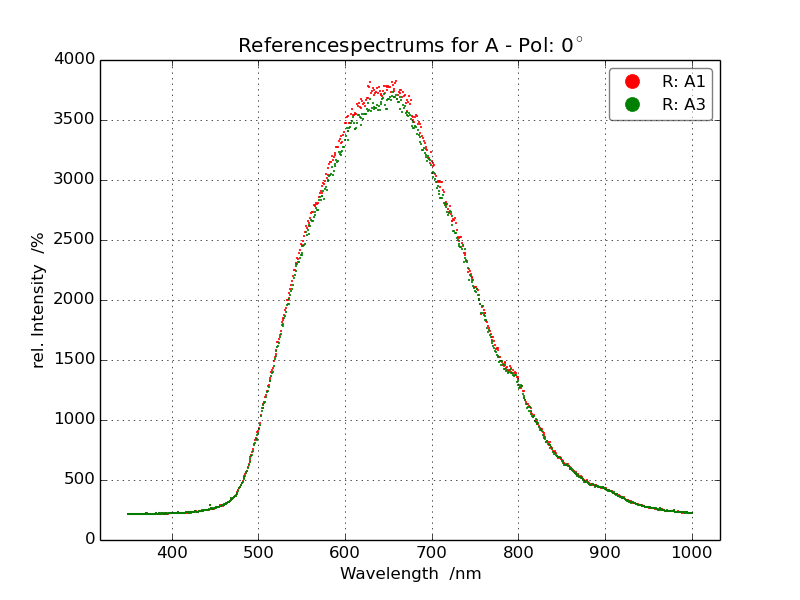
\includegraphics[width=\textwidth]{Figures/Refspec_APol0.png}
          \caption{Reference spectra for sample-column \textbf{A} at
              $\SI{0}{\degree}$ polarisation.}
          \label{fig:Refspec_APol0}
        \end{minipage}\\
        \begin{minipage}{.92\textwidth}
          \centering
          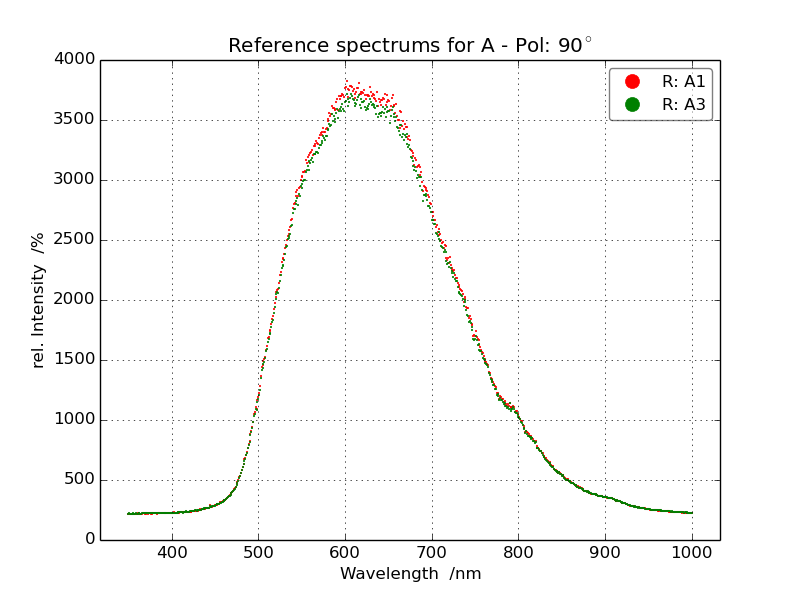
\includegraphics[width=\textwidth]{Figures/Refspec_APol90.png}
          \caption{Reference spectra for sample-column \textbf{A} at
              $\SI{90}{\degree}$ polarisation.}
          \label{fig:Refspec_APol90}
        \end{minipage}
      \end{figure}
      \newpage
      \begin{figure}[ht!]
        \centering
        \begin{minipage}{.92\textwidth}
          \centering
          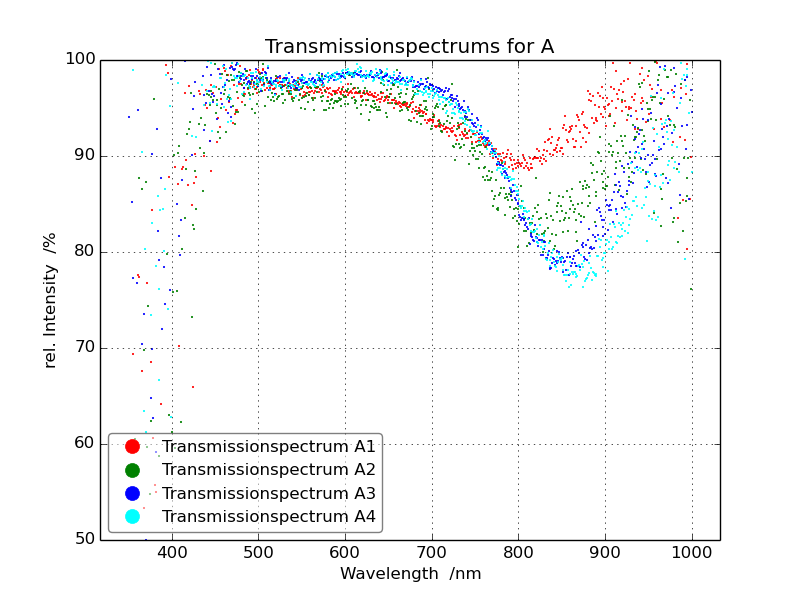
\includegraphics[width=\textwidth]{Figures/TransspecRAW_APol0.png}
          \caption{Data for sample-column \textbf{A} at $\SI{0}{\degree}$
              polarisation.}
          \label{fig:TransspecRAW_APol0}
        \end{minipage}\\
        \begin{minipage}{.92\textwidth}
          \centering
          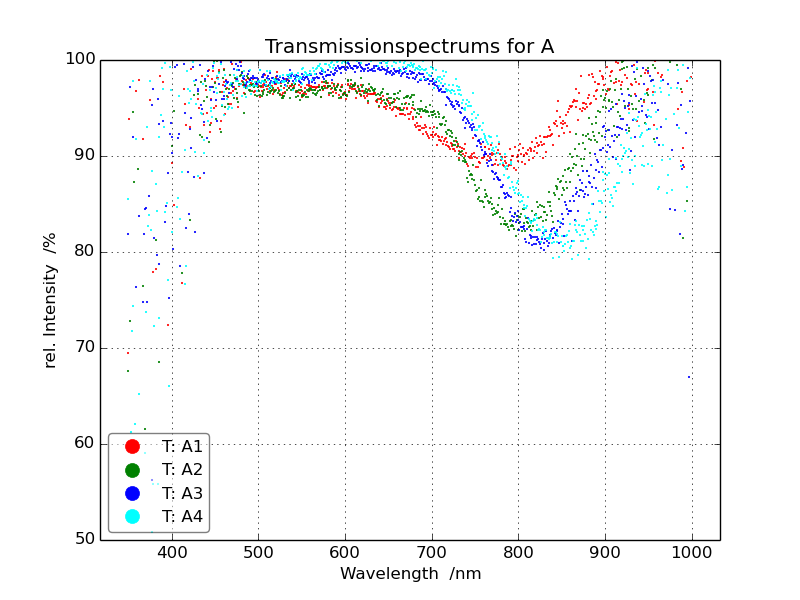
\includegraphics[width=\textwidth]{Figures/TransspecRAW_APol90.png}
          \caption{Data for sample-column \textbf{A} at $\SI{90}{\degree}$
              polarisation.}
          \label{fig:TransspecRAW_APol90}
        \end{minipage}
      \end{figure}
      
    \end{section}
    %%%%%%%%%%%%%%%%%%%%%%%%%%%%%%
    
    
    
    \newpage
    %%%%%%%%%%%%%%%%%%%%%%%%%%%%%%
    %%%%%%%%%%%%%%%%%%%%%%%%%%%%%%
    %%%%%%%%%%%%%%%%%%%%%%%%%%%%%%
    \begin{section}{Column \textbf{B}}
      \label{Appendix:DataB}
      
      \begin{figure}[ht!]
        \centering
        \begin{minipage}{.92\textwidth}
          \centering
          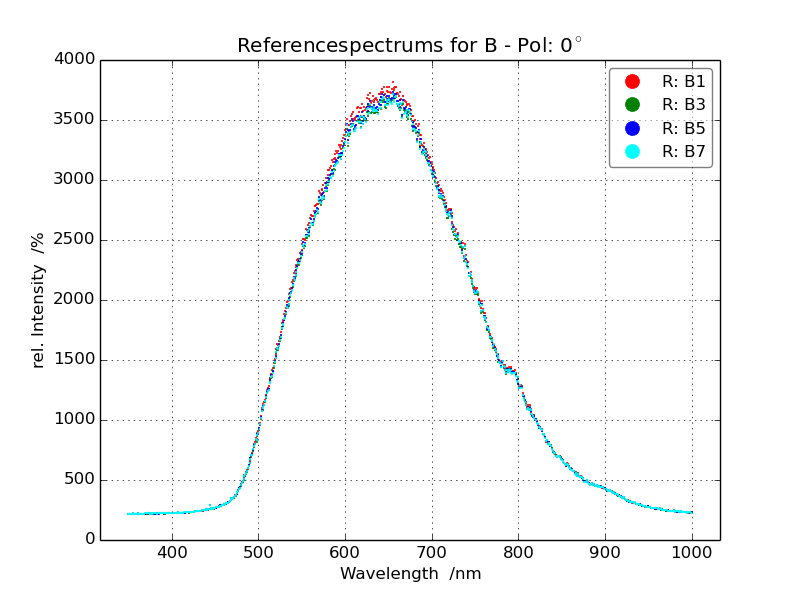
\includegraphics[width=\textwidth]{Figures/Refspec_BPol0.png}
          \caption{Reference spectra for sample-column \textbf{B} at
              $\SI{0}{\degree}$ polarisation.}
          \label{fig:Refspec_BPol0}
        \end{minipage}\\
        \begin{minipage}{.92\textwidth}
          \centering
          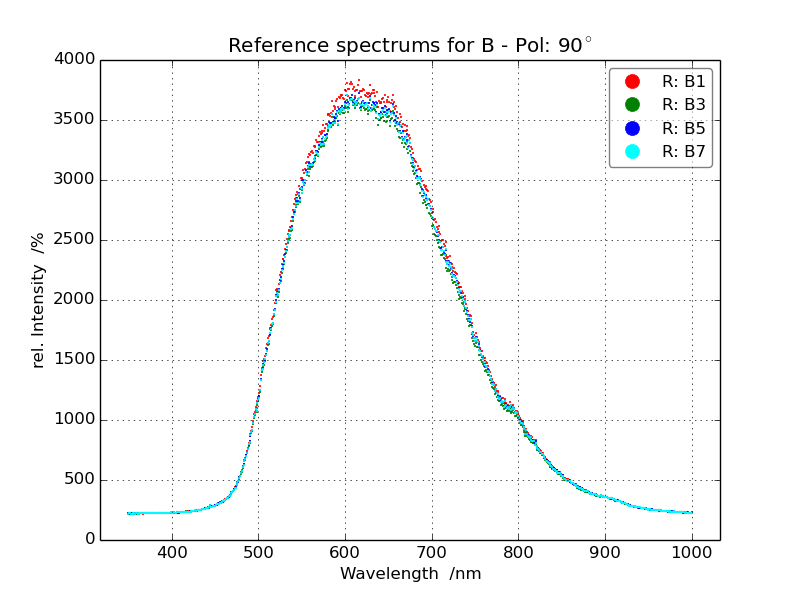
\includegraphics[width=\textwidth]{Figures/Refspec_BPol90.png}
          \caption{Reference spectra for sample-column \textbf{B} at
              $\SI{90}{\degree}$ polarisation.}
          \label{fig:Refspec_BPol90}
        \end{minipage}
      \end{figure}
      \newpage
      \begin{figure}[ht!]
        \centering
        \begin{minipage}{.92\textwidth}
          \centering
          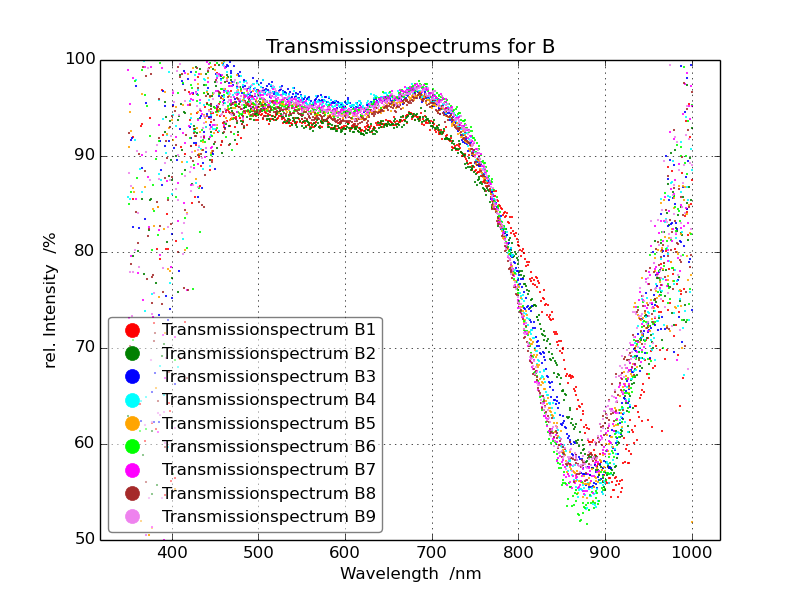
\includegraphics[width=\textwidth]{Figures/TransspecRAW_BPol0.png}
          \caption{Data for sample-column \textbf{B} at $\SI{0}{\degree}$
              polarisation.}
          \label{fig:TransspecRAW_BPol0}
        \end{minipage}\\
        \begin{minipage}{.92\textwidth}
          \centering
          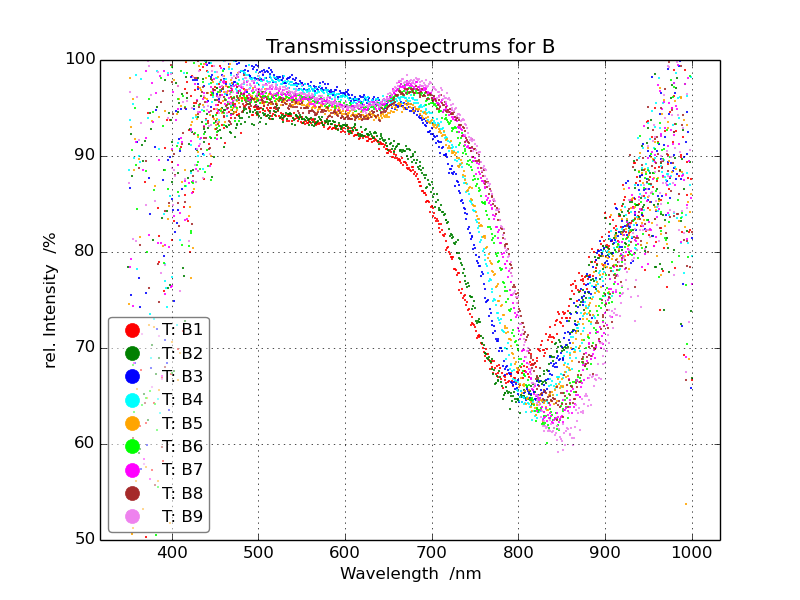
\includegraphics[width=\textwidth]{Figures/TransspecRAW_BPol90.png}
          \caption{Data for sample-column \textbf{B} at $\SI{90}{\degree}$
              polarisation.}
          \label{fig:TransspecRAW_BPol90}
        \end{minipage}
      \end{figure}
      
    \end{section}
    %%%%%%%%%%%%%%%%%%%%%%%%%%%%%%
    
    
    
    \newpage
    %%%%%%%%%%%%%%%%%%%%%%%%%%%%%%
    %%%%%%%%%%%%%%%%%%%%%%%%%%%%%%
    %%%%%%%%%%%%%%%%%%%%%%%%%%%%%%
    \begin{section}{Column \textbf{C}}
      \label{Appendix:DataC}
      
      \begin{figure}[ht!]
        \centering
        \begin{minipage}{.92\textwidth}
          \centering
          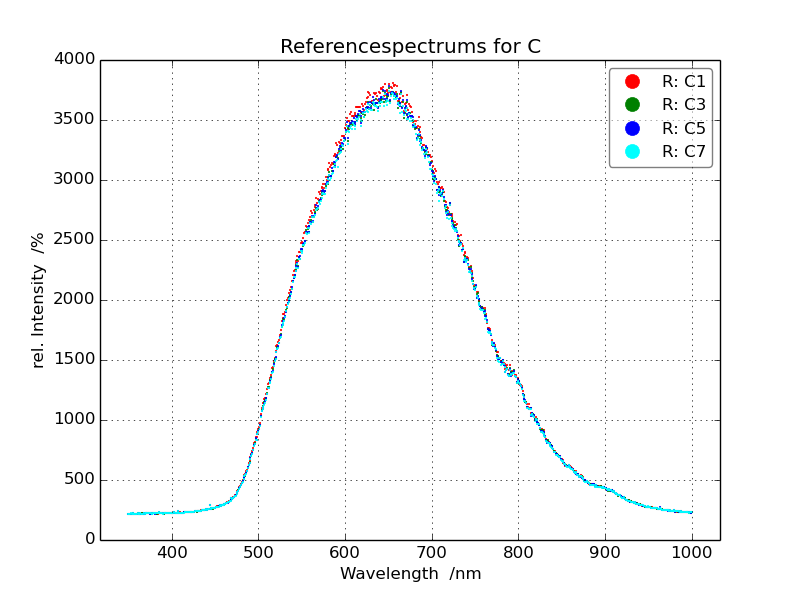
\includegraphics[width=\textwidth]{Figures/Refspec_CPol0.png}
          \caption{Reference spectra for sample-column \textbf{C} at
              $\SI{0}{\degree}$ polarisation.}
          \label{fig:Refspec_CPol0}
        \end{minipage}\\
        \begin{minipage}{.92\textwidth}
          \centering
          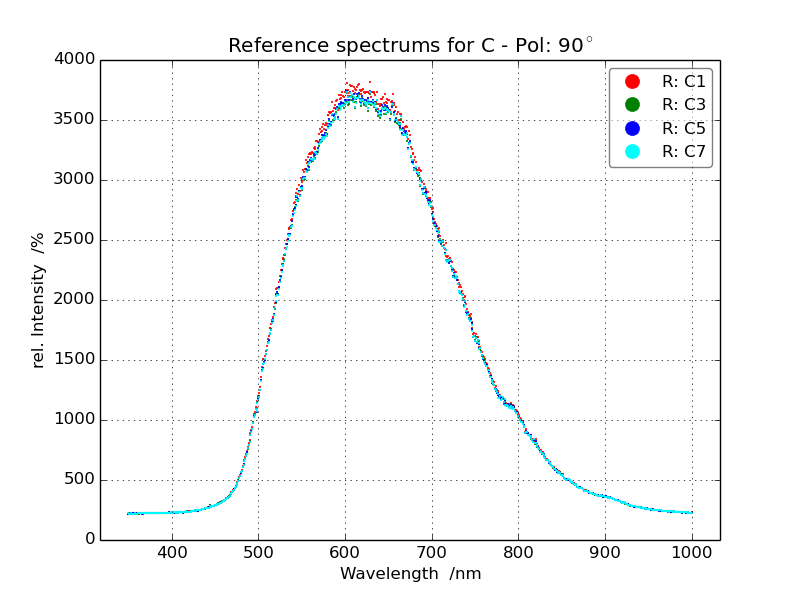
\includegraphics[width=\textwidth]{Figures/Refspec_CPol90.png}
          \caption{Reference spectra for sample-column \textbf{C} at
              $\SI{90}{\degree}$ polarisation.}
          \label{fig:Refspec_CPol90}
        \end{minipage}
      \end{figure}
      \newpage
      \begin{figure}[ht!]
        \centering
        \begin{minipage}{.92\textwidth}
          \centering
          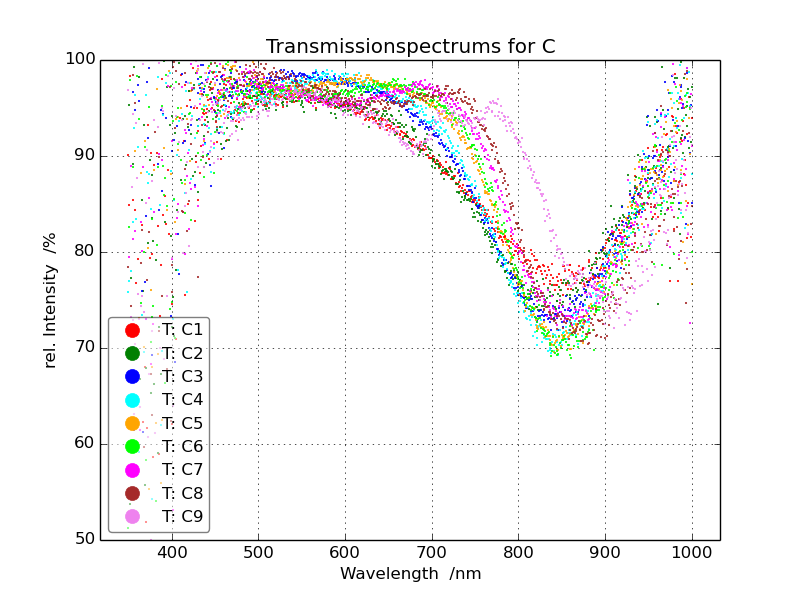
\includegraphics[width=\textwidth]{Figures/TransspecRAW_CPol0.png}
          \caption{Data for sample-column \textbf{C} at $\SI{0}{\degree}$
              polarisation.}
          \label{fig:TransspecRAW_CPol0}
        \end{minipage}\\
        \begin{minipage}{.92\textwidth}
          \centering
          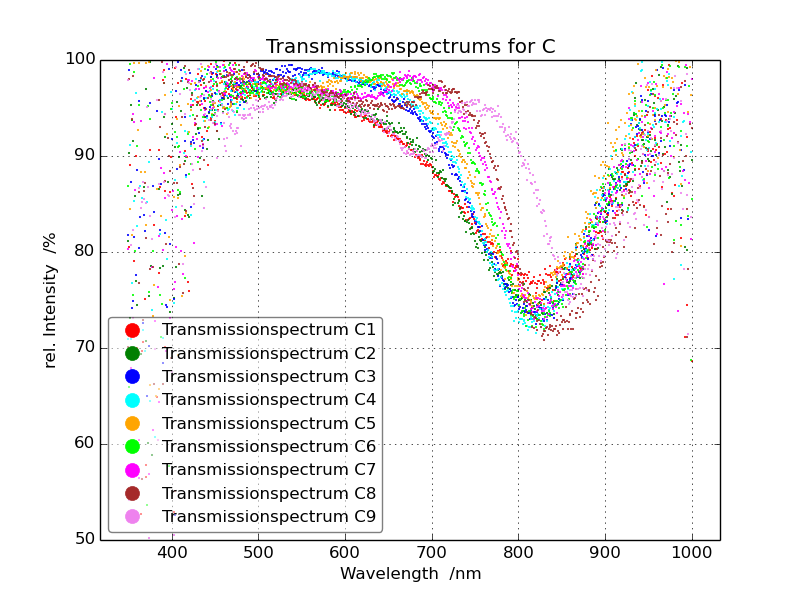
\includegraphics[width=\textwidth]{Figures/TransspecRAW_CPol90.png}
          \caption{Data for sample-column \textbf{C} at $\SI{90}{\degree}$
              polarisation.}
          \label{fig:TransspecRAW_CPol90}
        \end{minipage}
      \end{figure}
      
    \end{section}
    %%%%%%%%%%%%%%%%%%%%%%%%%%%%%%
    
    
    
    \newpage
    %%%%%%%%%%%%%%%%%%%%%%%%%%%%%%
    %%%%%%%%%%%%%%%%%%%%%%%%%%%%%%
    %%%%%%%%%%%%%%%%%%%%%%%%%%%%%%
    \begin{section}{Column \textbf{D}}
      \label{Appendix:DataD}
      
      \begin{figure}[ht!]
        \centering
        \begin{minipage}{.92\textwidth}
          \centering
          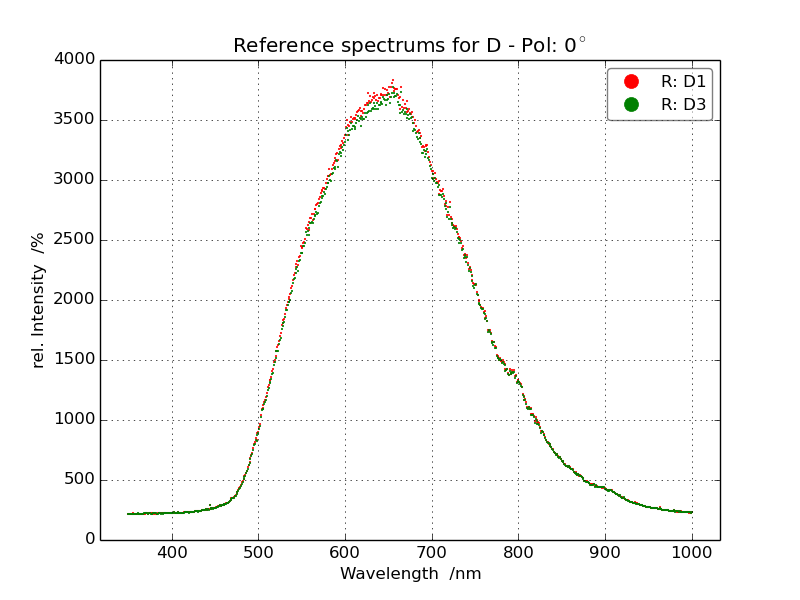
\includegraphics[width=\textwidth]{Figures/Refspec_DPol0.png}
          \caption{Reference spectra for sample-column \textbf{D} at
              $\SI{0}{\degree}$ polarisation.}
          \label{fig:Refspec_DPol0}
        \end{minipage}\\
        \begin{minipage}{.92\textwidth}
          \centering
          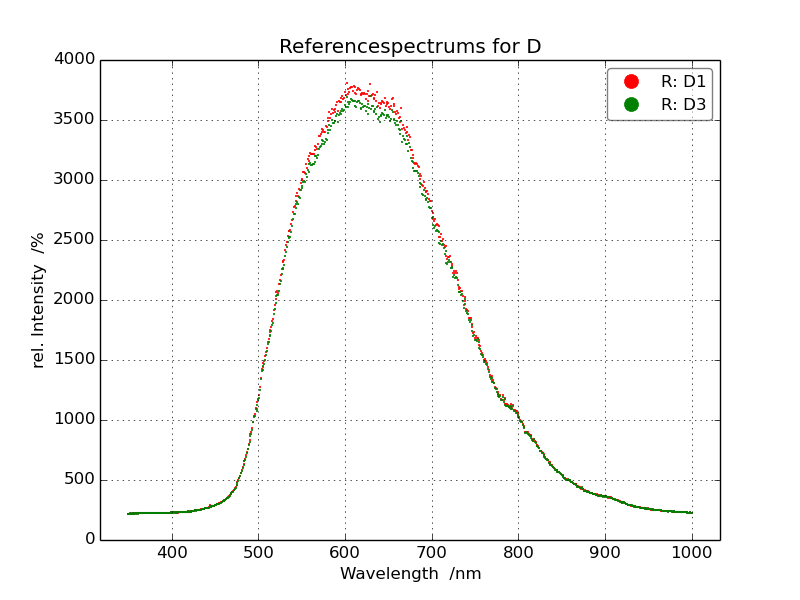
\includegraphics[width=\textwidth]{Figures/Refspec_DPol90.png}
          \caption{Reference spectra for sample-column \textbf{D} at
              $\SI{90}{\degree}$ polarisation.}
          \label{fig:Refspec_DPol90}
        \end{minipage}
      \end{figure}
      \newpage
      \begin{figure}[ht!]
        \centering
        \begin{minipage}{.92\textwidth}
          \centering
          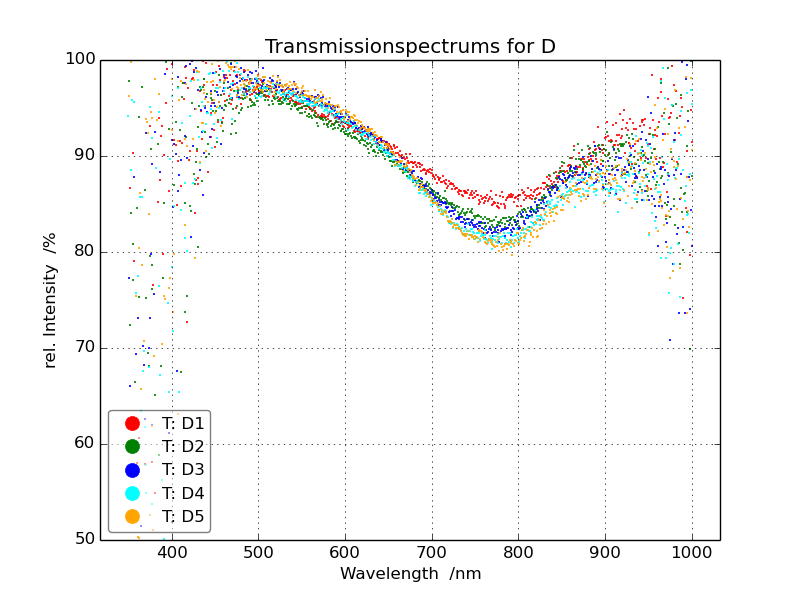
\includegraphics[width=\textwidth]{Figures/TransspecRAW_DPol0.png}
          \caption{Data for sample-column \textbf{D} at $\SI{0}{\degree}$
              polarisation.}
          \label{fig:TransspecRAW_DPol0}
        \end{minipage}\\
        \begin{minipage}{.92\textwidth}
          \centering
          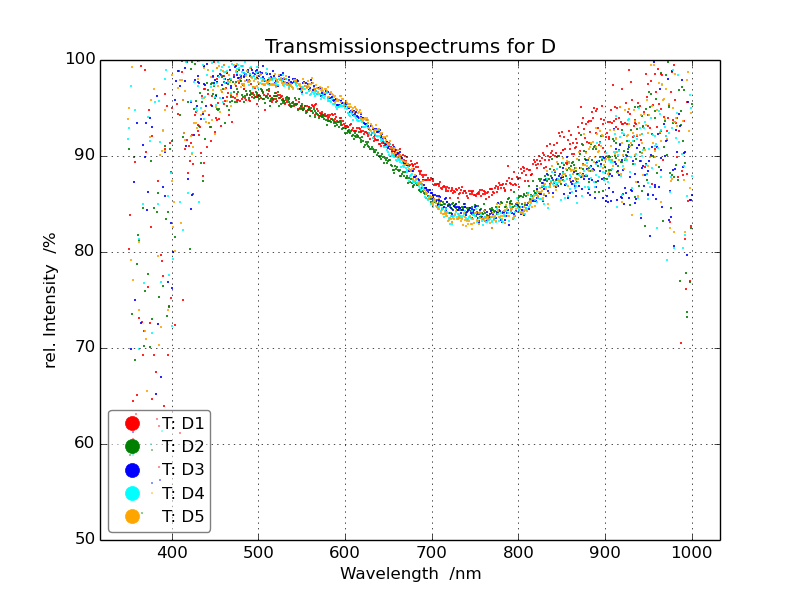
\includegraphics[width=\textwidth]{Figures/TransspecRAW_DPol90.png}
          \caption{Data for sample-column \textbf{D} at $\SI{90}{\degree}$
              polarisation.}
          \label{fig:TransspecRAW_DPol90}
        \end{minipage}
      \end{figure}
      
    \end{section}
    %%%%%%%%%%%%%%%%%%%%%%%%%%%%%%
    
    
    
    \newpage
    %%%%%%%%%%%%%%%%%%%%%%%%%%%%%%
    %%%%%%%%%%%%%%%%%%%%%%%%%%%%%%
    %%%%%%%%%%%%%%%%%%%%%%%%%%%%%%
    \begin{section}{Column \textbf{E}}
      \label{Appendix:DataE}
      
      \begin{figure}[ht!]
        \centering
        \begin{minipage}{.92\textwidth}
          \centering
          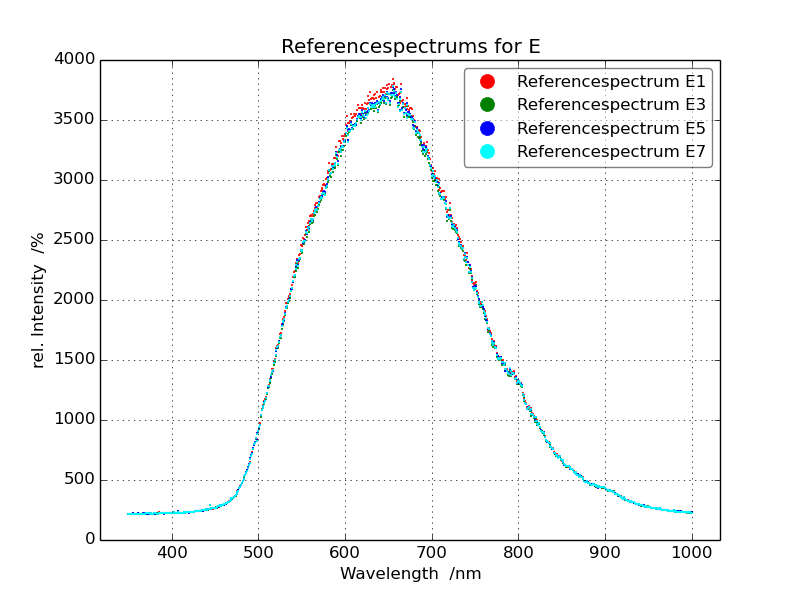
\includegraphics[width=\textwidth]{Figures/Refspec_EPol0.png}
          \caption{Reference spectra for sample-column \textbf{E} at
              $\SI{0}{\degree}$ polarisation.}
          \label{fig:Refspec_EPol0}
        \end{minipage}\\
        \begin{minipage}{.92\textwidth}
          \centering
          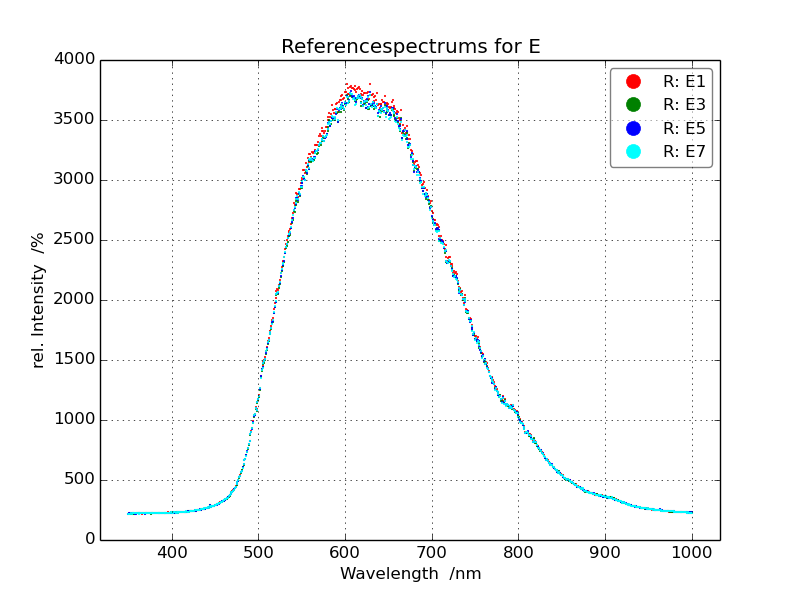
\includegraphics[width=\textwidth]{Figures/Refspec_EPol90.png}
          \caption{Reference spectra for sample-column \textbf{E} at
              $\SI{90}{\degree}$ polarisation.}
          \label{fig:Refspec_EPol90}
        \end{minipage}
      \end{figure}
      \newpage
      \begin{figure}[ht!]
        \centering
        \begin{minipage}{.92\textwidth}
          \centering
          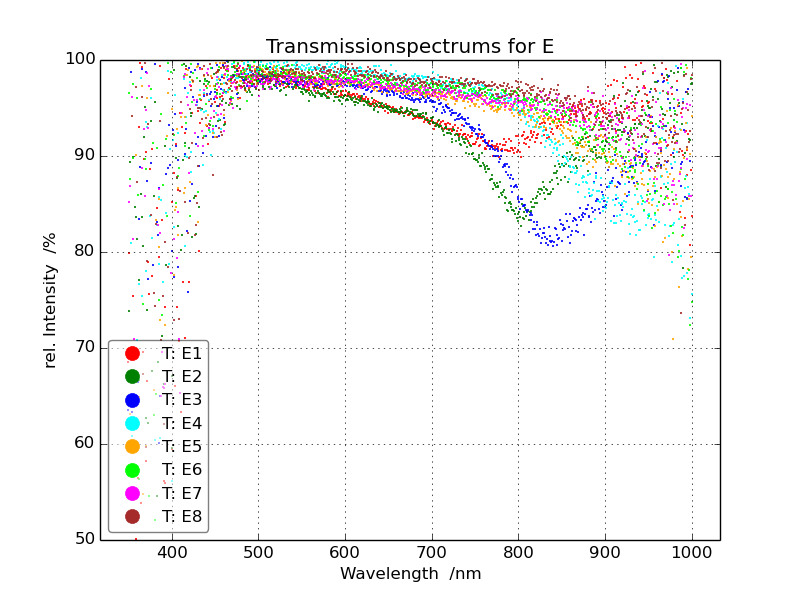
\includegraphics[width=\textwidth]{Figures/TransspecRAW_EPol0.png}
          \caption{Data for sample-column \textbf{E} at $\SI{0}{\degree}$
              polarisation.}
          \label{fig:TransspecRAW_EPol0}
        \end{minipage}\\
        \begin{minipage}{.92\textwidth}
          \centering
          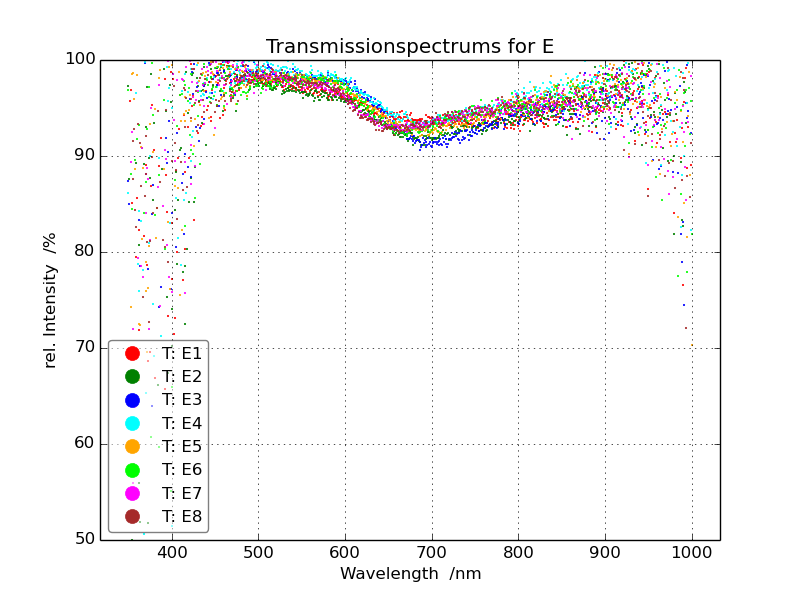
\includegraphics[width=\textwidth]{Figures/TransspecRAW_EPol90.png}
          \caption{Data for sample-column \textbf{E} at $\SI{90}{\degree}$
              polarisation.}
          \label{fig:TransspecRAW_EPol90}
        \end{minipage}
      \end{figure}
      
    \end{section}
    %%%%%%%%%%%%%%%%%%%%%%%%%%%%%%
    
  \end{chapter}
  %%%%%%%%%%%%%%%%%%%%%%%%%%%%%%
  
\end{appendix}
%%%%%%%%%%%%%%%%%%%%
 
  %%%%%%%%%%%%%%%%%%%%
  
  
  
  %%%%%%%%%%%%%%%%%%%%
  %%%%%%%%%%%%%%%%%%%%
  %%%%%%%%%%%%%%%%%%%%
  \begin{thebibliography}{99}
    \scriptsize
    
   
  \end{thebibliography}
  %%%%%%%%%%%%%%%%%%%%
 
\end{document}
%%%%%%%%%%
